% Akulin--Karlov. Batch 02, revision v2. Source: R36 CP02 and original scans.
% Editable geometry: source semantics first; no raster is embedded in this drawing.
\documentclass[border=5pt]{standalone}
\usepackage{fontspec,unicode-math}
\setmainfont{Noto Serif}
\setsansfont{Noto Sans}
\setmathfont{STIXTwoMath-Regular.otf}
\usepackage{tikz}
\usetikzlibrary{arrows.meta,calc,intersections,decorations.markings}
\definecolor{ScienceInk}{HTML}{000000}
\definecolor{ScienceCurve}{HTML}{000000}
\tikzset{
 axis/.style={draw=ScienceInk,line width=.70pt,-{Latex[length=2.2mm,width=1.25mm]}},
 baseline/.style={draw=ScienceInk,line width=.70pt},
 trace/.style={draw=ScienceCurve,line width=1.8pt,line cap=round,line join=round},
 level/.style={draw=ScienceInk,line width=2.1pt,line cap=butt},
 virtual/.style={draw=ScienceInk,line width=1.15pt,dash pattern=on 4pt off 3pt},
 photon/.style={draw=ScienceCurve,line width=1.05pt,-{Latex[length=2.25mm,width=1.35mm]},line cap=round},
 channel/.style={draw=ScienceCurve,line width=1.05pt,-{Latex[length=2.25mm,width=1.35mm]},line cap=round},
 dim/.style={draw=ScienceInk,line width=.70pt,-{Latex[length=1.8mm,width=1.1mm]}},
 lab/.style={text=ScienceInk,font=\fontsize{15}{18}\selectfont,inner sep=2pt},
 ticklab/.style={text=ScienceInk,font=\fontsize{13}{16}\selectfont\itshape,inner sep=1pt},
 levlab/.style={text=ScienceInk,font=\fontsize{14}{17}\selectfont,inner sep=2pt},
 panel/.style={text=ScienceInk,font=\fontsize{16}{19}\selectfont\itshape,inner sep=1pt}}
\pagestyle{empty}
\begin{document}

% Source: printed p.112. Same five-photon ladder as 9.5.
% Added channels start at |2,-1> and end at |2,-2>,...,|2,-5> (same bare level).
% Short outgoing branches on U2/U3/U4 are the author's continuation marks,
% NOT complete transitions to invented states. See REVIEW_NOTES.md.
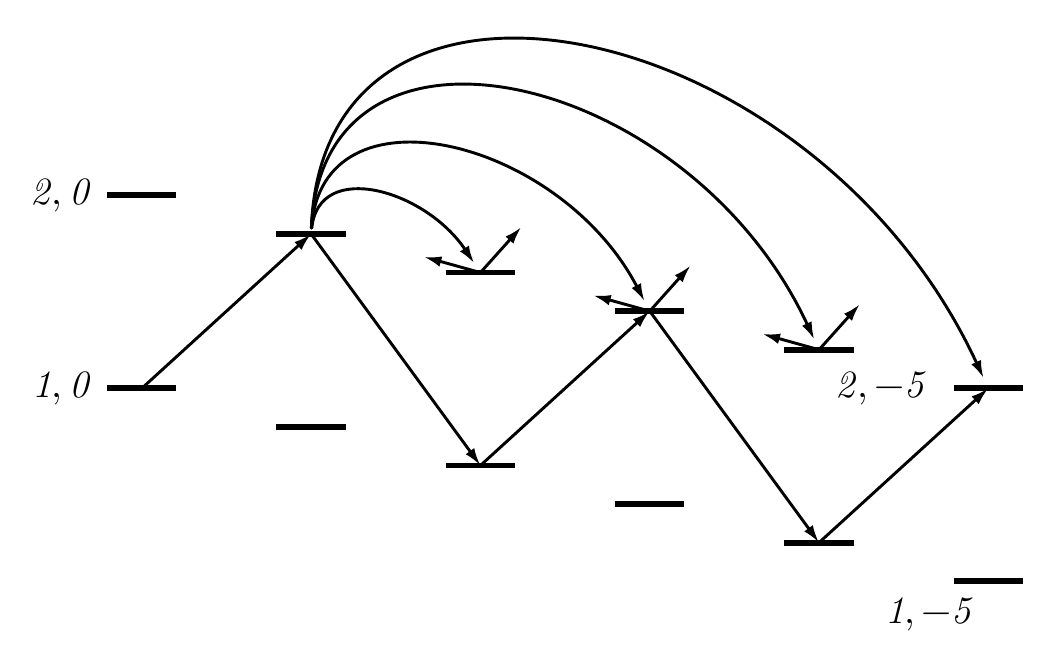
\begin{tikzpicture}[x=1cm,y=1cm]
\def\Photon{1}\def\Eone{0}\pgfmathsetmacro\Etwo{5*\Photon}
\def\Base{3.00}\def\Es{.49}\def\Xzero{1.1}\def\DX{2.15}
\foreach \k in {0,...,5}{
 \pgfmathsetmacro\xc{\Xzero+\k*\DX}
 \pgfmathsetmacro\lo{\Base+\Es*(\Eone-\k*\Photon)}
 \pgfmathsetmacro\hi{\Base+\Es*(\Etwo-\k*\Photon)}
 \coordinate (L\k) at (\xc,\lo);\coordinate (U\k) at (\xc,\hi);
 \draw[level] ({\xc-.44},\lo)--({\xc+.44},\lo);
 \draw[level] ({\xc-.44},\hi)--({\xc+.44},\hi);
}
\node[levlab,anchor=east] at (.53,5.45) {$\mathit{2,0}$};
\node[levlab,anchor=east] at (.53,3) {$\mathit{1,0}$};
\node[levlab,anchor=east] at ($(U5)+(-.70,0)$) {$\mathit{2,-5}$};
\node[levlab,anchor=north east] at ($(L5)+(-.1,-.13)$) {$\mathit{1,-5}$};
\foreach \from/\to in {L0/U1,U1/L2,L2/U3,U3/L4,L4/U5}{\draw[photon] (\from)--(\to);}
% Four distinct high arcs; each terminates on a different, physically named state.
\draw[channel,shorten <=2.2pt,shorten >=4pt] (U1) .. controls ($(U1)+(.10,.95)$) and ($(U2)+(-.70,1.05)$) .. (U2);
\draw[channel,shorten <=2.2pt,shorten >=4pt] (U1) .. controls ($(U1)+(.13,1.95)$) and ($(U3)+(-1.15,2.20)$) .. (U3);
\draw[channel,shorten <=2.2pt,shorten >=4pt] (U1) .. controls ($(U1)+(.14,3.15)$) and ($(U4)+(-1.65,3.55)$) .. (U4);
\draw[channel,shorten <=2.2pt,shorten >=4pt] (U1) .. controls ($(U1)+(.15,4.10)$) and ($(U5)+(-2.20,4.75)$) .. (U5);
% Continuation arrows are attached to their source levels, rather than floating.
\foreach \k in {2,3,4}{
 \draw[channel] (U\k)--($(U\k)+(-.72,.20)$);
 \draw[channel] (U\k)--($(U\k)+(.52,.58)$);
}
\pgfresetboundingbox
\path[use as bounding box] (-.35,-.10) rectangle (12.40,7.58);
\end{tikzpicture}

\end{document}
